% REV00 Tue 20 Jul 2021 08:12:01 WIB
% START Tue 20 Jul 2021 08:12:01 WIB

\chapter{Sepuluh}

% 11
\begin{figure}[htbp]
% h: here, where the figure appears in the text (use can always just use [h] )
% t: top,  top of the current page.
% b: bottom of the current page.
% p: page, top of the next available float space (sometimes end up being the end of the document).
\centerline{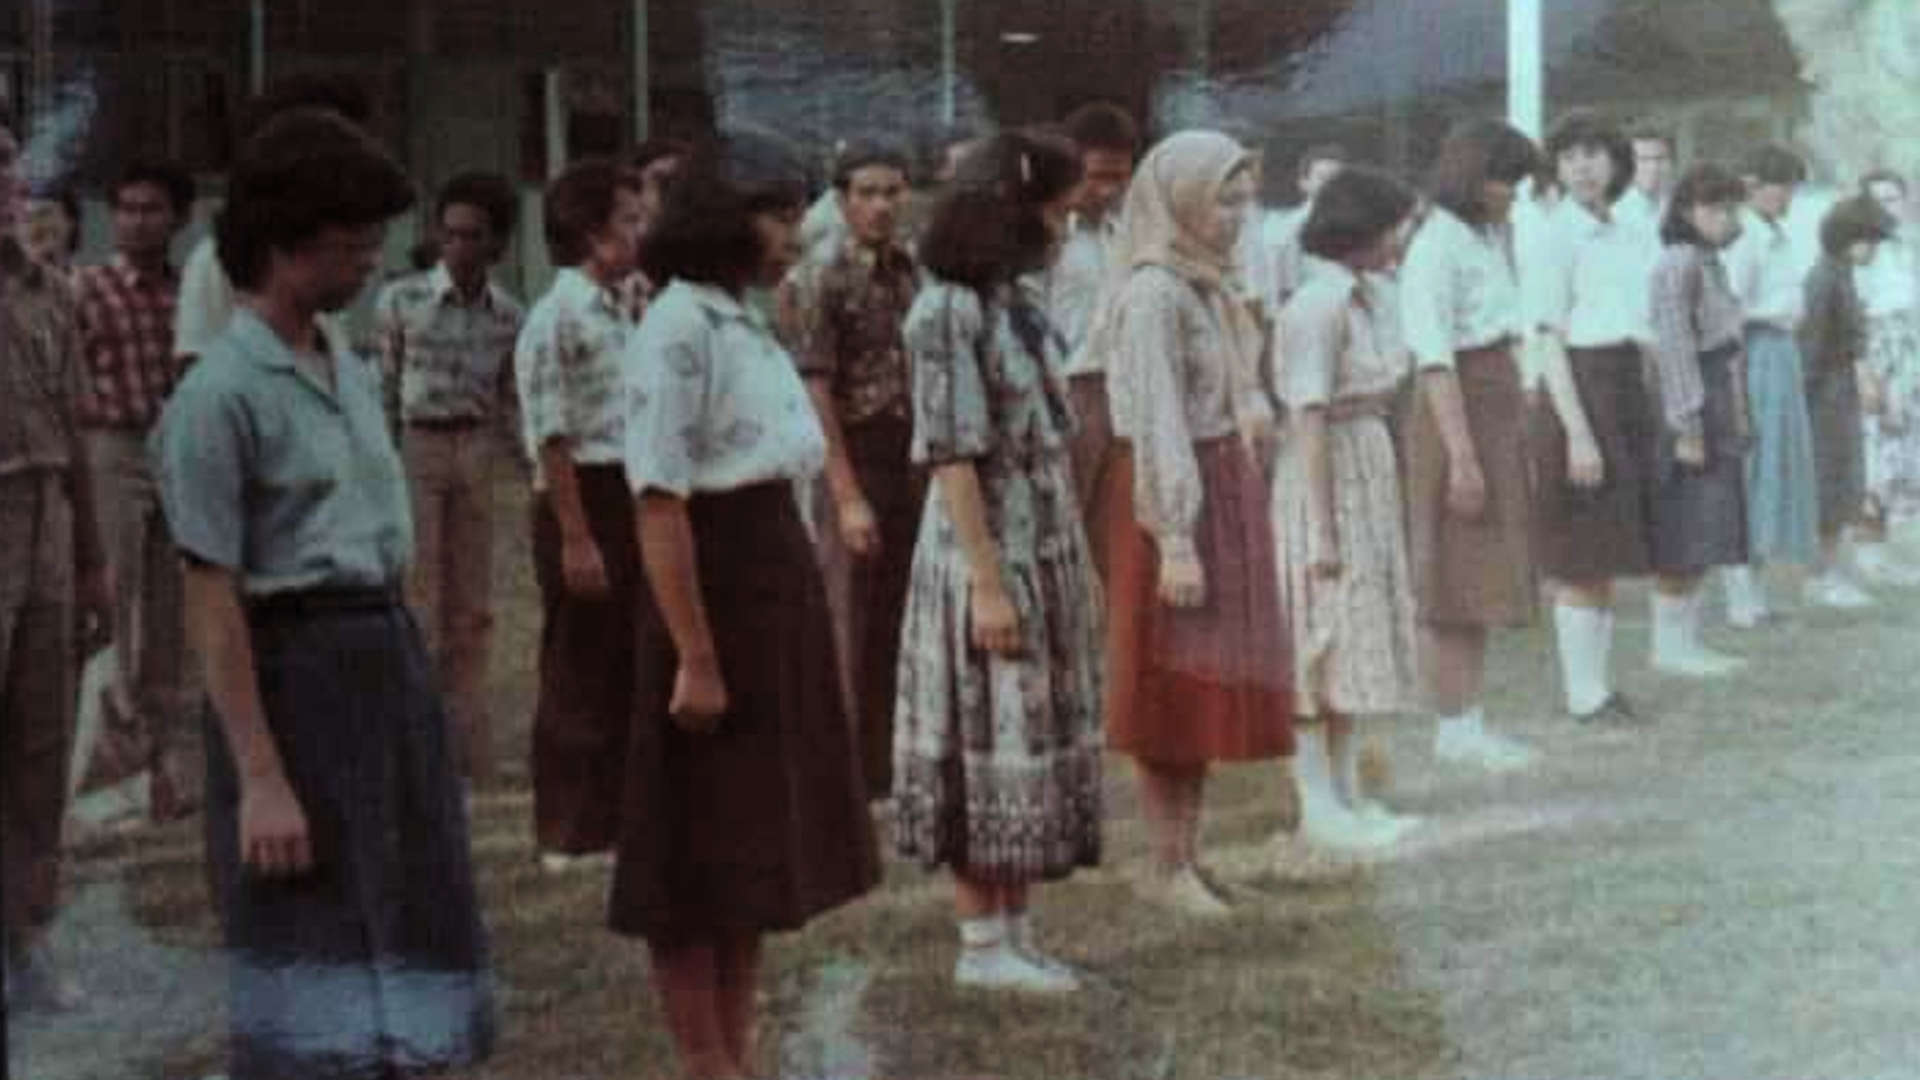
\includegraphics[scale=1.0]{01-10-01}}
\caption{Para Guru Besar/Profesor dan Doktor senior Fisika ITB saat ini,
pernah memuja Bang Satiri dengan wajib menyebut "Ya Dewaaaa..." sambil sujud simpuh di kakinya...
Asu tenan... Di foto ini terlihat Prof Triyanta Mugi, ada Prof Idam Arif, ada Prof Toto Winata,
ada Prof Zaki Suud, ada Prof Budi Mulyanti, ada Dr Siti Nurul, ada Dr. Neni, ada Dr. Pepen Arifin,
Dr. Ariadne... (Udjianto)}
\label{01-10-01}
\end{figure}
%

Ada suatu masa dia lagi-lagi menggunakan cap himpunan untuk membeli sepeda motor anyar, Honda Astrea. Alasannya, dana untuk penelitian tugas akhir. Masuk akal. Mana ada kelian berani kek gini kan?

“Lagian capek kan Bandung-Jakarta naik bus melulu..” ujarnya kepadaku. Iya, aku ingat, dulu kalau mau cepat kita harus pilih bus yang sopirnya rada gila: Lorena. Bus lain butuh 5 jm, Lorena hanya 3,5 jam saja.

Begitu bus berada di luar kota, entah dari Bandung atau Jakarta, bus kehilangan remnya. Duh…. Sopir hanya menginjaknya sekali, ketika mau belok ke restoran padang Pagi-Sore di kawasan Cipanas, Puncak. Sreeet…

Hanya butuh waktu dua puluh tiga menit buat istirahat makan di restoran padang itu. Bus pun melanjutkan perjalanan dengan damai. Tenang untuk seperokoan. Setelah itu, ya wuuuushhh… Rem diinjak untuk kedua kalinya ketika memasuki kawasan kota.

Pilihan untuk mendapatkan sepeda motor jadi lumayan masuk akal. Atau akal-akalan. Sama saja kan? Bagimanapun, saya pernah sekali digonceng Bang Tiri naik motor anyarnya itu dari Bandung ke Jakarta. Dan saya diantar sampai depan pintu rumah. Alhamdulillah…

Tanggal 25 Agustus 1985. Malam itu Ellyas Pical petinju kebanggaan kita merangsek mengalahkan petinju Australia, Wayne Mulholland: mempertahankan gelar sebagai juara IBF kelas bantam yunior. Horeee…

% 11
\begin{figure}[htbp]
% h: here, where the figure appears in the text (use can always just use [h] )
% t: top,  top of the current page.
% b: bottom of the current page.
% p: page, top of the next available float space (sometimes end up being the end of the document).
\centerline{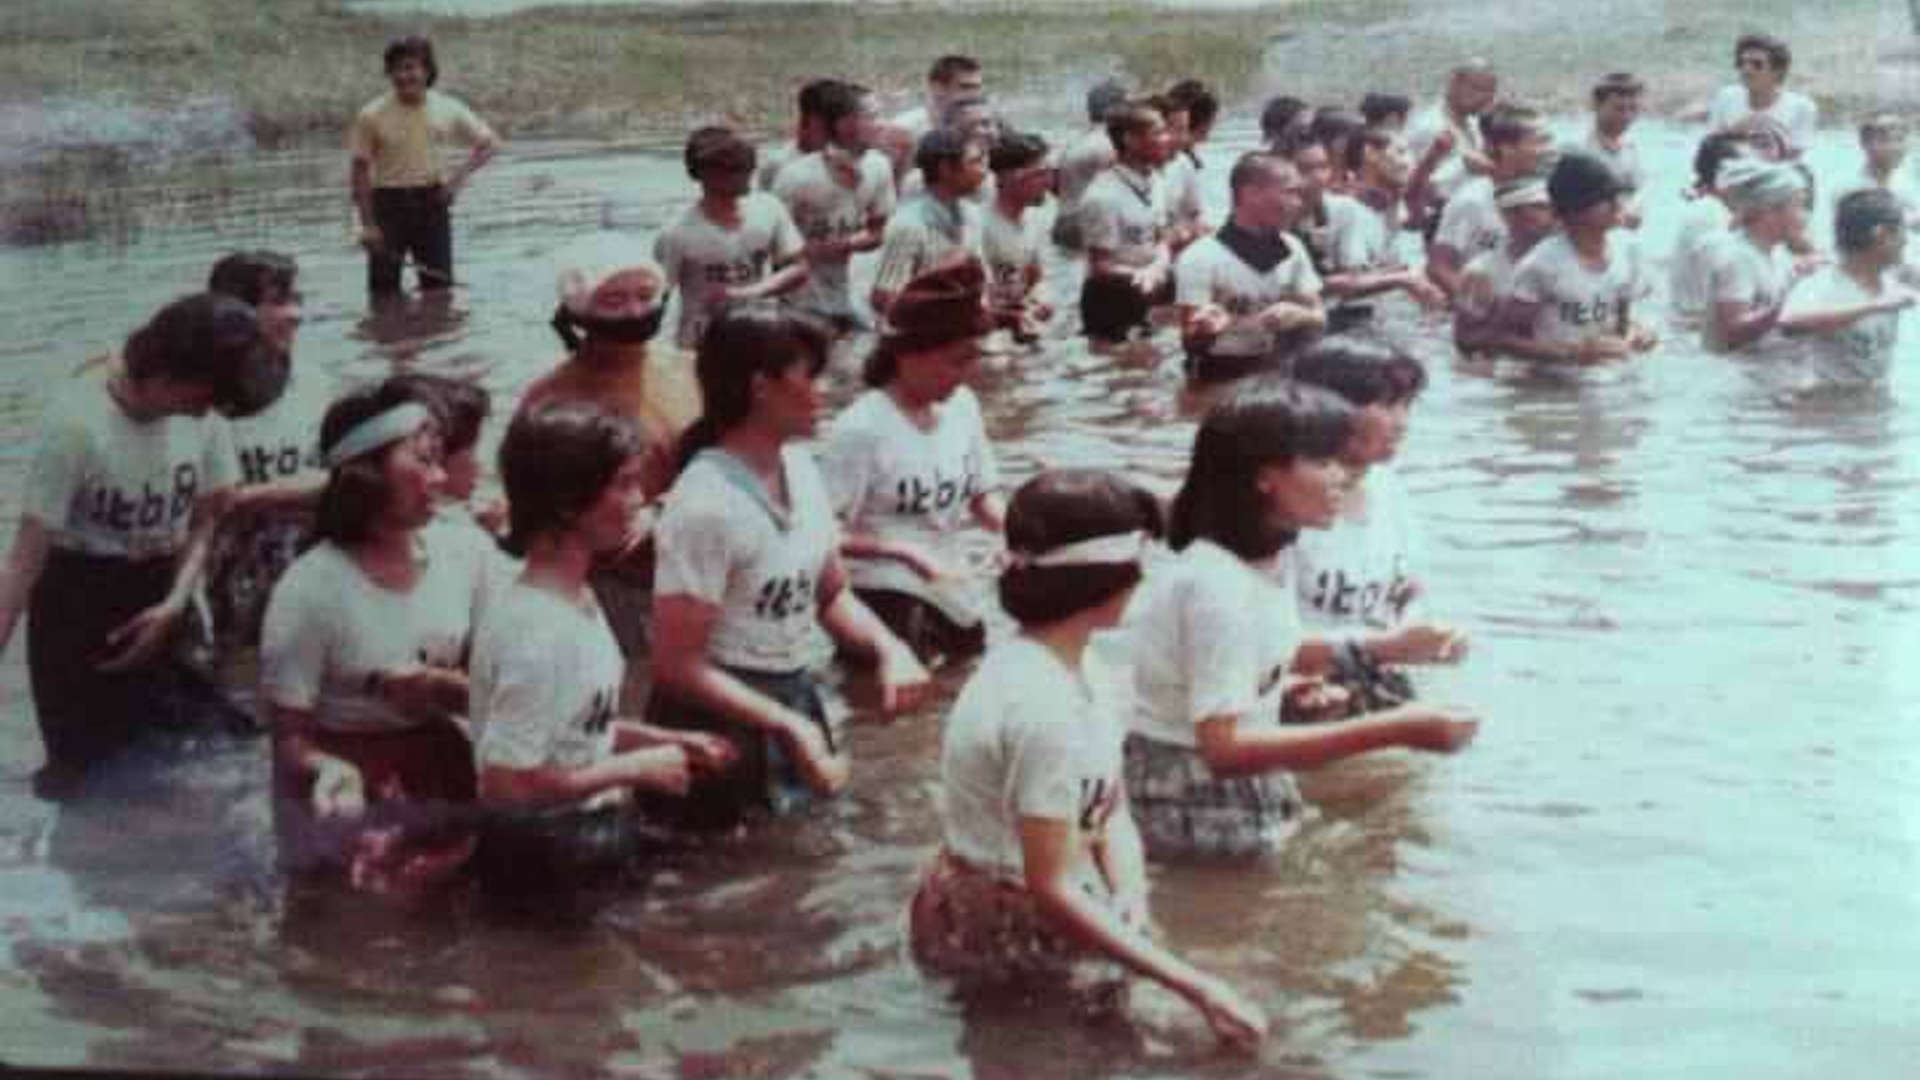
\includegraphics[scale=1.0]{01-10-02}}
\caption{Aku dan angkatanku (FI-81) menjadi korban perdana kekonyolan Bang Sat satu ini.... Assu tenan..!!
Ini salah satu foto penderitaan kami di Situ Patenggang, 
yg dinginnya membuat 'manuk' mengkeret berbulan-bulan... (Udjianto)}
\label{01-10-02}
\end{figure}
%

Malam itu juga Honda Astrea Bang Tiri ditilep maling. Pas kita bersama-sama bersorak-sorak menyemangati Ellyas Pical melalui TV. Astaghfirullah…

(Belakangan Bang Sat dengan kesadarannya sendiri membayar semua kenakalan ini dengan biaya tunai puluhan atau bahkan ratusan kali lipat!)

Sepeda motor sudah lenyap. Laporan ke Polisi buat apa juga dibuat. Padahal, Satiri terpaksa harus lebih sering ke Bandung untuk mengerjakan tugas akhir. Skripsi.

Selain itu, kita mulai belajar bahasa pemrograman komputer: Basic, Fortran dan juga Pascal. Saat sedang asik-asiknya belajar bahasa Pascal, lahirlah putrinya yang kedua, dan langsung ia beri nama dengan embel-embel “Fiska Pascali”.

Another amazingly beautiful name!

Waktu mencatatkan nama anaknya di kelurahan, bertanyalah si petugas yang juga orang Betawi:

“Ini anak elo namanya apaan, PAS LAKI?” (What is this your daughter name? PAS LAKI = fit for men?)

“Ampun bang… itu bacanya pas-ca-li… Sini aye yang nulis dah ya…”. (OMG. You have to read it as Pas-ca-li. Let me write it for you…). Dasar Betawi!

Selesai dengan urusan aneh itu., dia segera balik ke Bandung, mengerjakan tugas akhir. Apa tugas akhir yang bisa cepat lulus?

Bikin alat!

Tugas akhir ini kalau kita terpeleset maka akan menjadi tugas tanpa akhir! Ada seorang sobat yang semua mata kuliah bisa diselesaikannya dalam empat tahun, namun dia butuh tambahan 5 tahun lagi untuk menyelesaikan tugas ‘tanpa’ akhirnya itu. Lulus juga dia…

Ada juga sahabat yang lain, yang mengerjakan desain tugas akhir dengan berkutat sendirian di rumah selama tiga bulan penuh. Namun ketika dia menemui pembimbingnya, sang profesor mengatakan dengan entengnya bahwa topik itu sudah ada orang lain yang mengerjakannya. Langsung deh sobatku yang satu ini memutuskan untuk tidak perlu lulus dari ITB. Antik. Tapi kemudian hidupnya berhasil dan sejahtera.

Satiri membuat alat untuk mendeteksi level ketinggian cairan di dalam tabung tertutup. Kalau sekarang, alat seperti tinggal kita beli saja di toko bangunan atau toko elektronika.

Ya, ‘ELEKTRONIKA’. Masih ingat kan salah satu magic words yang ia tanyakan kepada Bang Ipul, gurunya yang pertama? Malaikat dan Tuhan tidak pernah salah dalam mencatat.

Kata-kata itu adalah doa!

***

Pada saat itu hubungan Bang Tiri dengan mertuanya sudah berbeda 180 derajat. Balik arah, menjadi menantu kesayangan.

Satiri tidak pernah melakukan perlawanan, dia hanya bertahan dan menunjukkan kasih sayang dan tekad kuatnya membangun masa depan. Babanya Fitria pun menjadi paham arti menjadi mahasiswa ITB.

Terlebih-lebih ketika Kelvy Safira lahir. Bayi mungil cantik alang kepalang, melebihi ibu-bapaknya, dan selalu tersenyum. Cobalah bayangkan, kakek atau nenek mana yang tidak akan luluh melihatnya?

Terkadang kita terlalu takut dalam menentukan pilihan hidup. Padahal kita sudah hafal bahwa di balik setiap kesulitian pasti ada kemudahan.

***

Ketika hampir menyelesaikan tugas akhirnya itu, di suatu musim hujan yang dingin Satiri bertanya kepada saya:

“Ren, ini ada tawaran untuk jadi dosen di Universitas Brawijaya (UB) Malang, menurutmu bagaimana?”

Saya terpukau juga atas pertanyaan itu. Sebab, yang saya kerjakan saat itu masih jauh dari tugas akhir. Saya masih berjuang untuk lulus beberapa mata pelajaran tahun ke-3!

Tapi mungkin Satiri menghargai pilihan saya untuk lebih aktif di kegiatan sosial dan budaya, daripada belajar Fisika. Karena sejuknya hujan, saya pun bisa berpikir cukup bagus sehingga tahu arah pertanyaan dia.

“Aku kira bagus juga jadi dosen. Bisa dikirim kuliah ke luar negeri, dan juga tetap bisa mengerjakan proyek-proyek di swasta. Bisa lah jadi orang kaya. Kesempatan bagus, ambil saja.”

“Iya sih… Ini kalau kita ambil, kita akan segera dikursuskan bahasa Inggris enam bulan di Kampus, dikasih uang saku juga. Dan, katanya akan langsung dikirim ke Australia?”

AUSTRALIA? Anda tentu ingat, itu kan salah satu dari kata-kata ajaib yang ia tanyakan kepada Mas Paijo, gurunya yang kedua?

Wah, kejadian ini…

Walaupun Satiri kurang yakin jadi dosen akan bikin kaya, kesempatan itu diambilnya juga. Ternyata dari Fisika ada dua orang yang ikut program calon dosen UB ini. Kursus sudah dimulai walaupun mereka belum dinyatakan lulus dan diwisuda. (Sobat yang bersamanya itu belakangan malah menjadi profesor kenamaan di universitas ternama di Sulawesi, kampung halamannya)

Suatu ketika, di jeda kursus, mereka berdua diminta datang ke Rektorat UB. Di sana sudah menunggu 20 orang dosen senior, dan rapat pun dibuka oleh Pak Rektor.

“Bapak-bapak dosen senior yang saya hormati, kita akan segera mendapat tambahan dua orang dosen baru, macan-macan dari kampus ITB. Ini saya perkenalkan mereka…”

“Ya ampun, macaaan… tambah gede dah kepala gua”, pikir Satiri. (“Gosh. I guess my head is getting bigger…”)

Betulkah ‘elektronika’ membawa Satiri ke ‘Australia’? 
\\[10pt]

Sumber tulisan asli \url{https://www.facebook.com/reno.alamsyah.94/posts/10226555102769891}

